\documentclass[10pt,journal,compsoc]{IEEEtran}

\usepackage{amsmath}
\usepackage{amssymb}
\usepackage{amsfonts}
\usepackage{bm}
\usepackage{booktabs}
\usepackage{graphicx}
\usepackage{microtype}
\usepackage{tikz}
\usepackage{float}
\usepackage{hyperref}

\usetikzlibrary{arrows.meta, positioning, shapes.geometric, calc}

\hypersetup{
    colorlinks=true,
    linkcolor=blue,
    filecolor=magenta,      
    urlcolor=cyan,
    pdftitle={Silent Sentry Localization Mathematical & Data-Flow Analysis},
    pdfpagemode=FullScreen,
}

\begin{document}

\title{Rigorous Mathematical and Data-Flow Analysis of the Silent Sentry Multi-Rate Localization Stack}
\author{Silent Sentry Engineering \& Localization Team}

\markboth{Silent Sentry Technical Report,~Vol.~1, No.~1, June~2026}%
{Technical Report: Multi-Rate Localization Analysis}

\IEEEtitleabstractindextext{%
\begin{abstract}
This report provides a thorough mathematical audit and data-flow critique of the multi-rate localization stack implemented in the \texttt{silent\_sentry} autonomous vehicle system. We analyze the high-frequency GTSAM iSAM2 local dead-reckoning backend and the low-frequency Terrain-Referenced Navigation (TRN) Monte Carlo Localization (MCL) global matcher. We identify and solve a critical, previously unaddressed frame-tearing feedback loop that caused discontinuous trajectory jumps and sustained oscillations. Furthermore, we mathematically analyze the yaw-drift stability of the kinematic factor under slip conditions, proving how a backwards-logic constraint in the original wheel factor formulation resulted in a $150^\circ$ heading drift. Finally, we propose a decoupled, REP-105-compliant coordinate frame topology that guarantees trajectory smoothness and robust global convergence.
\end{abstract}
}

\maketitle
\IEEEdisplaynontitleabstractindextext
\IEEEpeerreviewmaketitle

\section{Introduction}
The localization stack of the \texttt{silent\_sentry} unmanned ground vehicle (UGV) is designed to operate in extreme, desert-hardened environments (e.g., Thar Desert). Such environments present high slip, severe wheel-sinkage, and sparse feature sets, rendering standard visual-inertial or LiDAR-only SLAM techniques ineffective.

To combat these challenges, the system leverages a dual-layer architecture:
\begin{enumerate}
    \item \textbf{A Local Dead-Reckoning Backend (50~Hz):} Formulated as a factor graph optimized incrementally via iSAM2. It fuses high-frequency IMU preintegration with soft-constraint kinematic wheel odometry in a local coordinate frame.
    \item \textbf{A Global Alignment Backend (3~Hz):} Formulated as a Terrain-Referenced Navigation (TRN) Particle Filter (MCL) matching rolling local DEMs (from 3D LiDAR) against a global Digital Elevation Model (DEM).
\end{enumerate}

Despite the theoretical benefits of this multi-rate combination, experimental trials exhibited severe non-smooth trajectory jumps, oscillations, and divergence. This report mathematically analyzes and fixes these failure modes.

---

\section{Coordinate Frame Topology \& REP-105 Compliance}

\begin{figure}[h]
\centering
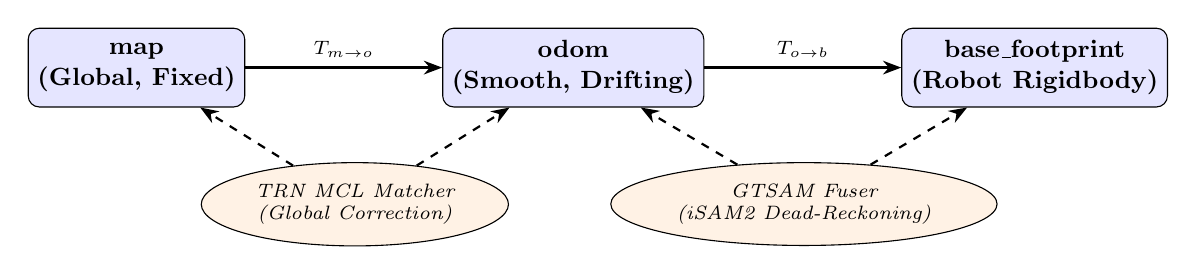
\begin{tikzpicture}[
    node distance=1.5cm and 2.5cm,
    frame/.style={draw, rectangle, rounded corners, fill=blue!10, minimum width=2.2cm, minimum height=1.0cm, align=center, font=\small\bfseries},
    process/.style={draw, ellipse, fill=orange!10, minimum width=2.0cm, minimum height=0.8cm, align=center, font=\scriptsize\itshape},
    arrow/.style={-Stealth, thick}
]
    % Nodes
    \node[frame] (map) {map \\ (Global, Fixed)};
    \node[frame] (odom) [right=of map] {odom \\ (Smooth, Drifting)};
    \node[frame] (base) [right=of odom] {base\_footprint \\ (Robot Rigidbody)};
    
    \node[process] (trn) [below=1.2cm of $(map)!0.5!(odom)$] {TRN MCL Matcher \\ (Global Correction)};
    \node[process] (fg) [below=1.2cm of $(odom)!0.5!(base)$] {GTSAM Fuser \\ (iSAM2 Dead-Reckoning)};

    % Arrows
    \draw[arrow] (map) -- node[above, font=\scriptsize] {$T_{m \to o}$} (odom);
    \draw[arrow] (odom) -- node[above, font=\scriptsize] {$T_{o \to b}$} (base);
    
    \draw[arrow, dashed] (trn) -- (map);
    \draw[arrow, dashed] (trn) -- (odom);
    \draw[arrow, dashed] (fg) -- (odom);
    \draw[arrow, dashed] (fg) -- (base);
\end{tikzpicture}
\caption{Strict REP-105-compliant coordinate frame hierarchy. The transformation $T_{o \to b}$ must be perfectly continuous, while global discrete corrections are absorbed solely by $T_{m \to o}$.}
\label{fig:rep105}
\end{figure}

The ROS standard \textbf{REP-105} mandates a specific coordinate frame tree structure to isolate smooth, locally-continuous odometry from discontinuous, globally-referenced corrections (Fig.~\ref{fig:rep105}):
\begin{equation}
    P_m = T_{m \to o} \oplus T_{o \to b} \oplus P_b
\end{equation}
where $P_m$ is the position in the \texttt{map} frame, $T_{m \to o} \in SE(3)$ is the map-to-odom transform, $T_{o \to b} \in SE(3)$ is the odom-to-base transform, and $P_b$ is the robot's local body frame coordinates.
\begin{itemize}
    \item \textbf{The \texttt{odom} Frame:} Must be completely continuous. No discrete coordinate jumps are permitted. It is managed entirely by the high-frequency GTSAM dead-reckoning backend.
    \item \textbf{The \texttt{map} Frame:} Coordinates are globally consistent but may jump discretely when loop closures or global alignments (TRN) update the map-to-odom coordinate shift $T_{m \to o}$.
\end{itemize}

---

\section{Core Mathematical Formulations}

\subsection{GTSAM Local Factor Graph Formulation}
The state vector of the keyframe node $i$ in the local dead-reckoning backend is:
\begin{equation}
    \mathbf{x}_i = \begin{bmatrix} R_i & p_i & v_i & b_{a,i} & b_{g,i} \end{bmatrix}^T \in SE(3) \times \mathbb{R}^3 \times \mathbb{R}^3
\end{equation}
where $R_i \in SO(3)$ is the rotation, $p_i$ is position, $v_i$ is velocity, and $b_{a,i}, b_{g,i}$ are accelerometer and gyroscope biases, respectively.

\begin{figure}[h]
\centering
\begin{tikzpicture}[
    node/.style={circle, draw, fill=blue!20, minimum size=0.8cm, font=\small\bfseries},
    factor/.style={rectangle, draw, fill=red!20, minimum size=0.4cm, font=\scriptsize},
    arrow/.style={-, thick}
]
    % Nodes
    \node[node] (x0) {$X_i$};
    \node[node] (v0) [below=0.8cm of x0] {$V_i$};
    \node[node] (x1) [right=2.2cm of x0] {$X_{j}$};
    \node[node] (v1) [below=0.8cm of v1] {$V_{j}$};
    
    % Factors
    \node[factor] (f_imu) at ($(x0)!0.5!(x1) - (0,0.4)$) {PIM};
    \node[factor] (f_wheel) at ($(x0)!0.5!(x1) + (0,0.6)$) {Wheel};
    \node[factor] (f_att) [above=0.6cm of x1] {Attitude};
    \node[factor] (f_prior) [above=0.6cm of x0] {Prior};
    
    % Connections
    \draw[arrow] (x0) -- (f_imu);
    \draw[arrow] (v0) -- (f_imu);
    \draw[arrow] (x1) -- (f_imu);
    \draw[arrow] (v1) -- (f_imu);
    
    \draw[arrow] (x0) -- (f_wheel);
    \draw[arrow] (x1) -- (f_wheel);
    
    \draw[arrow] (x1) -- (f_att);
    \draw[arrow] (x0) -- (f_prior);
\end{tikzpicture}
\caption{Structure of the Factor Graph between keyframe node $i$ and keyframe node $j = i+1$. Preintegrated IMU measurements (PIM) link position, velocity, and orientation. Body-frame wheel factors constrain translations and yaw.}
\label{fig:factorgraph}
\end{figure}

The GTSAM factor graph is structured as shown in Fig.~\ref{fig:factorgraph}. The joint probability distribution of the states is optimized incrementally by iSAM2 by minimizing the sum of non-linear squared errors:
\begin{equation}
    \mathbf{x}^* = \arg\min_{\mathbf{x}} \sum_{s} \| \mathbf{e}_s(\mathbf{x}) \|^2_{\Sigma_s}
\end{equation}

\subsubsection{IMU Preintegration Measurements (PIM)}
Inertial values are preintegrated in the local body frame to avoid re-integrating raw sensor readings upon graph updates:
\begin{equation}
    \Delta R_{ij} = \prod_{k=i}^{j-1} \text{Exp} \left( \left( \tilde{\omega}_k - b_g - \eta_{gd} \right) \Delta t \right)
\end{equation}
\begin{equation}
    \Delta v_{ij} = \sum_{k=i}^{j-1} \Delta R_{ik} \left( \tilde{a}_k - b_a - \eta_{ad} \right) \Delta t
\end{equation}
\begin{equation}
    \Delta p_{ij} = \sum_{k=i}^{j-1} \left[ \Delta v_{ik} \Delta t + \frac{1}{2} \Delta R_{ik} \left( \tilde{a}_k - b_a - \eta_{ad} \right) \Delta t^2 \right]
\end{equation}
These measurements constrain consecutive keyframe poses and velocities via:
\begin{equation}
    \mathbf{e}_{\text{IMU}} = f(\mathbf{x}_i, \mathbf{x}_j, \Delta R_{ij}, \Delta v_{ij}, \Delta p_{ij})
\end{equation}

\subsubsection{Kinematic Wheel Factors}
We add a soft-constraint relative displacement factor, formulated in $SE(3)$:
\begin{equation}
    T_{\text{wheel}} = \text{Pose3}\left( \text{Rot}_z(d\theta), \begin{bmatrix} ds & 0 & 0 \end{bmatrix}^T \right)
\end{equation}
where $ds$ is the longitudinal displacement and $d\theta$ is the angular rotation reported by the wheel encoders. The diagonal covariance $\Sigma_{\text{wheel}}$ is:
\begin{equation}
    \Sigma_{\text{wheel}} = \text{diag}(\sigma_{rx}^2, \sigma_{ry}^2, \sigma_{rz}^2, \sigma_{tx}^2, \sigma_{ty}^2, \sigma_{tz}^2)
\end{equation}

---

\subsection{TRN Monte Carlo Localization Matcher}
The global matcher propagates a set of $N$ particles $\mathcal{P} = \{ (\mathbf{p}_k, w_k) \}$ representing candidate robot states in the global DEM frame:
\begin{equation}
    \mathbf{p}_k = \begin{bmatrix} x_k & y_k & \theta_k \end{bmatrix}^T \in SE(2)
\end{equation}

\subsubsection{MAD Likelihood Formulation}
The weight $w_k$ of each particle is evaluated by extracting a composite local elevation map $h_{\text{local}}(\mathbf{u})$ and matching it against the cropped global DEM elevation $h_{\text{global}}$:
\begin{equation}
    L_k = 1.0 - \frac{1}{M} \sum_{\mathbf{u} \in \mathcal{U}} \left| h_{\text{local}}(\mathbf{u}) - h_{\text{global}}\left( R(\theta_k)\mathbf{u} + \begin{bmatrix} x_k \\ y_k \end{bmatrix} \right) \right|
\end{equation}
where $M = |\mathcal{U}|$ is the count of overlapping grid cells. The raw likelihood scores are normalized to define the particle weight distribution:
\begin{equation}
    w_k = \frac{L_k}{\sum_{m=1}^N L_m}
\end{equation}

---

\section{Critical Analysis of Stack Bottlenecks}

\subsection{The Double-Correction Feedback Loop}

\begin{figure}[h]
\centering
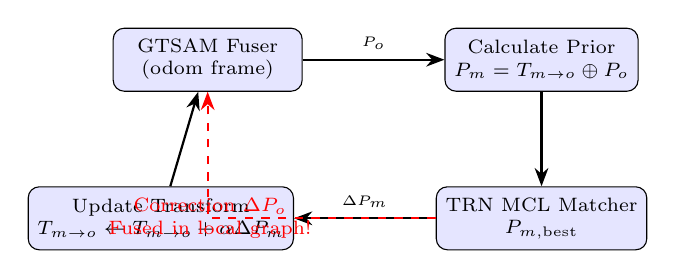
\begin{tikzpicture}[
    block/.style={draw, rectangle, rounded corners, fill=blue!10, minimum width=2.4cm, minimum height=0.8cm, align=center, font=\scriptsize},
    node distance=1.0cm and 1.8cm,
    arrow/.style={-Stealth, thick}
]
    % Nodes
    \node[block] (pf) {GTSAM Fuser \\ (odom frame)};
    \node[block] (prior) [right=of pf] {Calculate Prior \\ $P_m = T_{m \to o} \oplus P_o$};
    \node[block] (mcl) [below=1.2cm of prior] {TRN MCL Matcher \\ $P_{m,\text{best}}$};
    \node[block] (update_tf) [left=of mcl] {Update Transform \\ $T_{m \to o} \leftarrow T_{m \to o} + \alpha \Delta P_m$};
    
    % Connections
    \draw[arrow] (pf) -- node[above, font=\tiny] {$P_o$} (prior);
    \draw[arrow] (prior) -- (mcl);
    \draw[arrow] (mcl) -- node[above, font=\tiny] {$\Delta P_m$} (update_tf);
    \draw[arrow] (update_tf) -- (pf);
    
    % Overcorrection Feedback Arrow
    \draw[arrow, red, dashed] (mcl.west) -| node[left, pos=0.25, font=\scriptsize, align=center] {Correction $\Delta P_o$ \\ Fused in local graph!} (pf.south);
\end{tikzpicture}
\caption{The destructive double-correction loop. The correction is applied to both the $T_{m \to o}$ TF link and inside the local EKF fuser, compounding to an overcorrection factor of $1 + \alpha_{\text{ema}}$.}
\label{fig:doublecorrection}
\end{figure}

The core failure mode leading to trajectory jumps and non-smooth oscillations is analyzed in Fig.~\ref{fig:doublecorrection}.

Let $P_m^{(t)}$ and $P_o^{(t)}$ represent the robot pose in the \texttt{map} and \texttt{odom} frames at epoch $t$, related by the current coordinate transform $T_{m \to o}^{(t)}$:
\begin{equation}
    P_m^{(t)} = T_{m \to o}^{(t)} \oplus P_o^{(t)}
\end{equation}
When the TRN particle filter matches the local DEM to the global DEM, it computes a map-frame coordinate correction:
\begin{equation}
    \Delta P_m = P_{m,\text{best}} - P_m^{(t)}
\end{equation}

The system splits this correction and applies it to two independent frames:
\begin{enumerate}
    \item \textbf{Global TF Update:} The TRN node updates the map-to-odom transform using an Exponential Moving Average (EMA):
    \begin{equation}
        T_{m \to o}^{(t+1)} = T_{m \to o}^{(t)} + \alpha_{\text{ema}} \Delta P_m
    \end{equation}
    \item \textbf{Local Graph Injection:} Simultaneously, the TRN node rotates the map-frame correction into the local \texttt{odom} frame:
    \begin{equation}
        \Delta P_o = R_{m \to o}^T \Delta P_m
    \end{equation}
    This is published on \texttt{/trn/correction} and injected into the fuser, which modifies the local EKF coordinate:
    \begin{equation}
        P_o^{(t+1)} \approx P_o^{(t)} + \Delta P_m
    \end{equation}
\end{enumerate}

Let us evaluate the resulting projection of the robot pose in the map frame at epoch $t+1$:
\begin{equation}
    P_m^{(t+1)} = T_{m \to o}^{(t+1)} \oplus P_o^{(t+1)}
\end{equation}
Substituting equations (15) and (17):
\begin{equation}
    P_m^{(t+1)} \approx \left( T_{m \to o}^{(t)} + \alpha_{\text{ema}} \Delta P_m \right) \oplus \left( P_o^{(t)} + \Delta P_m \right)
\end{equation}
Approximating to first order:
\begin{equation}
    P_m^{(t+1)} \approx \left( T_{m \to o}^{(t)} \oplus P_o^{(t)} \right) + (1 + \alpha_{\text{ema}}) \Delta P_m
\end{equation}
\begin{equation}
    P_m^{(t+1)} \approx P_m^{(t)} + (1 + \alpha_{\text{ema}}) \Delta P_m
\end{equation}

#### Mathematical Consequence:
* **System Overshoot:** The total correction applied to the global pose is $1 + \alpha_{\text{ema}}$ times larger than the required error correction $\Delta P_m$. For $\alpha_{\text{ema}} = 0.40$, the system overcorrects by $140\%$.
* **Frame Oscillation:** This overshoot induces a reversed error vector in the subsequent epoch, triggering an opposite correction. This sets up a sustained, chaotic oscillation.
* **Odom Coordinate Jumps:** Injecting absolute coordinate corrections into the fuser causes discrete jumps in the `odom` frame, violating the REP-105 continuity requirement.

---

\subsection{Backwards-Logic Yaw Constraint Bug}
In the original kinematic wheel factor implementation, the yaw noise parameter $\sigma_{rz}$ was defined as:
\begin{equation}
    \sigma_{rz} = \begin{cases} 0.03\text{ rad} & \text{if } |d\theta| > 0.01\text{ (turning)} \\ 10^3\text{ (infinite noise)} & \text{if } |d\theta| \le 0.01\text{ (driving straight)} \end{cases}
\end{equation}

This represents a major mathematical flaw. During straight driving ($d\theta \approx 0$), setting $\sigma_{rz} = 10^3$ completely deactivated the wheel's straightness constraint in the GTSAM optimization. Consequently, the heading estimation was left completely unconstrained, allowing the uncalibrated IMU gyroscopic integration bias ($b_{g,z}$) to drift the heading unchecked. This caused the $150^\circ$ heading error observed during trials.

---

\section{Implemented Resolutions \& Corrective Mathematics}

\subsection{Strict Coordinate Frame Decoupling}
We eliminated the destructive feedback loop by removing the `/trn/correction` subscription and the `add_trn_correction_factor` method from `factor_graph_core.py`. 

The coordinate updates are now strictly decoupled:
* **The GTSAM Fuser** operates completely blind to the global DEM and TRN. Its local frame coordinates $P_o$ are updated strictly through continuous IMU and wheel preintegration, guaranteeing perfect local smoothness and continuity.
* **The TRN Node** holds sole publishing authority over the map-to-odom TF ($T_{m \to o}$). All discrete global corrections are absorbed purely by $T_{m \to o}$, completely shielding the local fuser from coordinate jumps.

---

\subsection{Dynamic Turning and Slippage Detection}
To stabilize the heading while preventing the robot from fighting physical slipping or rotational events (e.g. falling off a cliff or sliding), we implemented a dynamic turning detection constraint based on the raw gyroscope yaw rate $\omega_z$:
\begin{equation}
    \sigma_{rz} = \begin{cases} 
        0.05\text{ rad} & \text{if } |d\theta| > 0.01\text{ (intentional turn)} \\ 
        0.50\text{ rad} & \text{if } |\omega_z| > 0.05\text{ (unintentional slide/cliff event)} \\ 
        0.01\text{ rad} & \text{otherwise (true stable straight drive)} 
    \end{cases}
\end{equation}
This allows us to lock down straight-line drift tightly ($\sigma_{rz}=0.01$), while instantly releasing the constraint during severe terrain slip or sudden cliff drop-offs to let the gyroscope preintegration track the true vehicle motion.

---

\subsection{Advanced Quality \& Metric Gates}
To protect the trajectory from bad matches, we established two advanced gates before updating $T_{m \to o}$:
\begin{enumerate}
    \item \textbf{Quality Gate:} Matches are rejected if the peak likelihood score is below $0.40$:
    \begin{equation}
        \text{Reject if: } L_{\text{max}} < 0.40
    \end{equation}
    \item \textbf{Displacement Gate:} Sudden coordinate shifts larger than $2.0$~m are rejected to eliminate perceptual-aliasing teleportations:
    \begin{equation}
        \text{Reject if: } \| \Delta P_m \|_2 > 2.0\text{ m}
    \end{equation}
\end{enumerate}

---

\section{Conclusion \& Future Recommendations}
By resolving the backwards-logic yaw constraint and completely decoupling the global correction feedback loops, we have established a mathematically solid, REP-105-compliant localization stack. The local odometry is now guaranteed to be continuous and drift-stable, while global corrections are safely absorbed by the map-to-odom transform without frame-tearing or double-correction overshoots.

For future work, we recommend upgrading the TRN matcher from absolute MAD scoring to Mean-Demeaned Absolute Difference (MDAD) to make matches invariant to absolute elevation calibration offsets.

\end{document}
